\section{Methods}

\subsection{Participants}
20 participants(12 female, 8 male; all right-handed) from the local university community participated in the experiment. Their age ranged from 21 to 41 years. All participants were naive to the purpose of the experiment and had normal or corrected-to-normal vision. The experiment was approved by the ethics committee of the University of T\"ubingen, and was performed in accordance with the Declaration of Helsinki. Participants gave written informed consent prior to the experiment and were compensated with 8 Euro per hour for their participation. 

\subsection{Apparatus}
The virtual environment was displayed in stereo using an HTC Vive head-mounted-display (HMD) with a resolution of 1080 x 1200 pixels per eye (2160 x 1200 pixels combined). Inter-pupillary distance was measured with a pupilometer and set accordingly on the HTC Vive for each participant. Before the experiment two HTC Vive controllers were used to calibrate the experiment according to the participant's arm span. During the experiment one HTC Vive controller was attached to the participant's wrist to track hand and arm movements. The tracked controller movement data was used to display a virtual arm that moves according to the participants real movements. Participants were sitting during the whole experiment and viewed their virtual task in front of them. An XBox controller \ref{fig:xbox} was used in order to allow participants to make decisions and proceed to the next trial.

\begin{figure}
\centering
  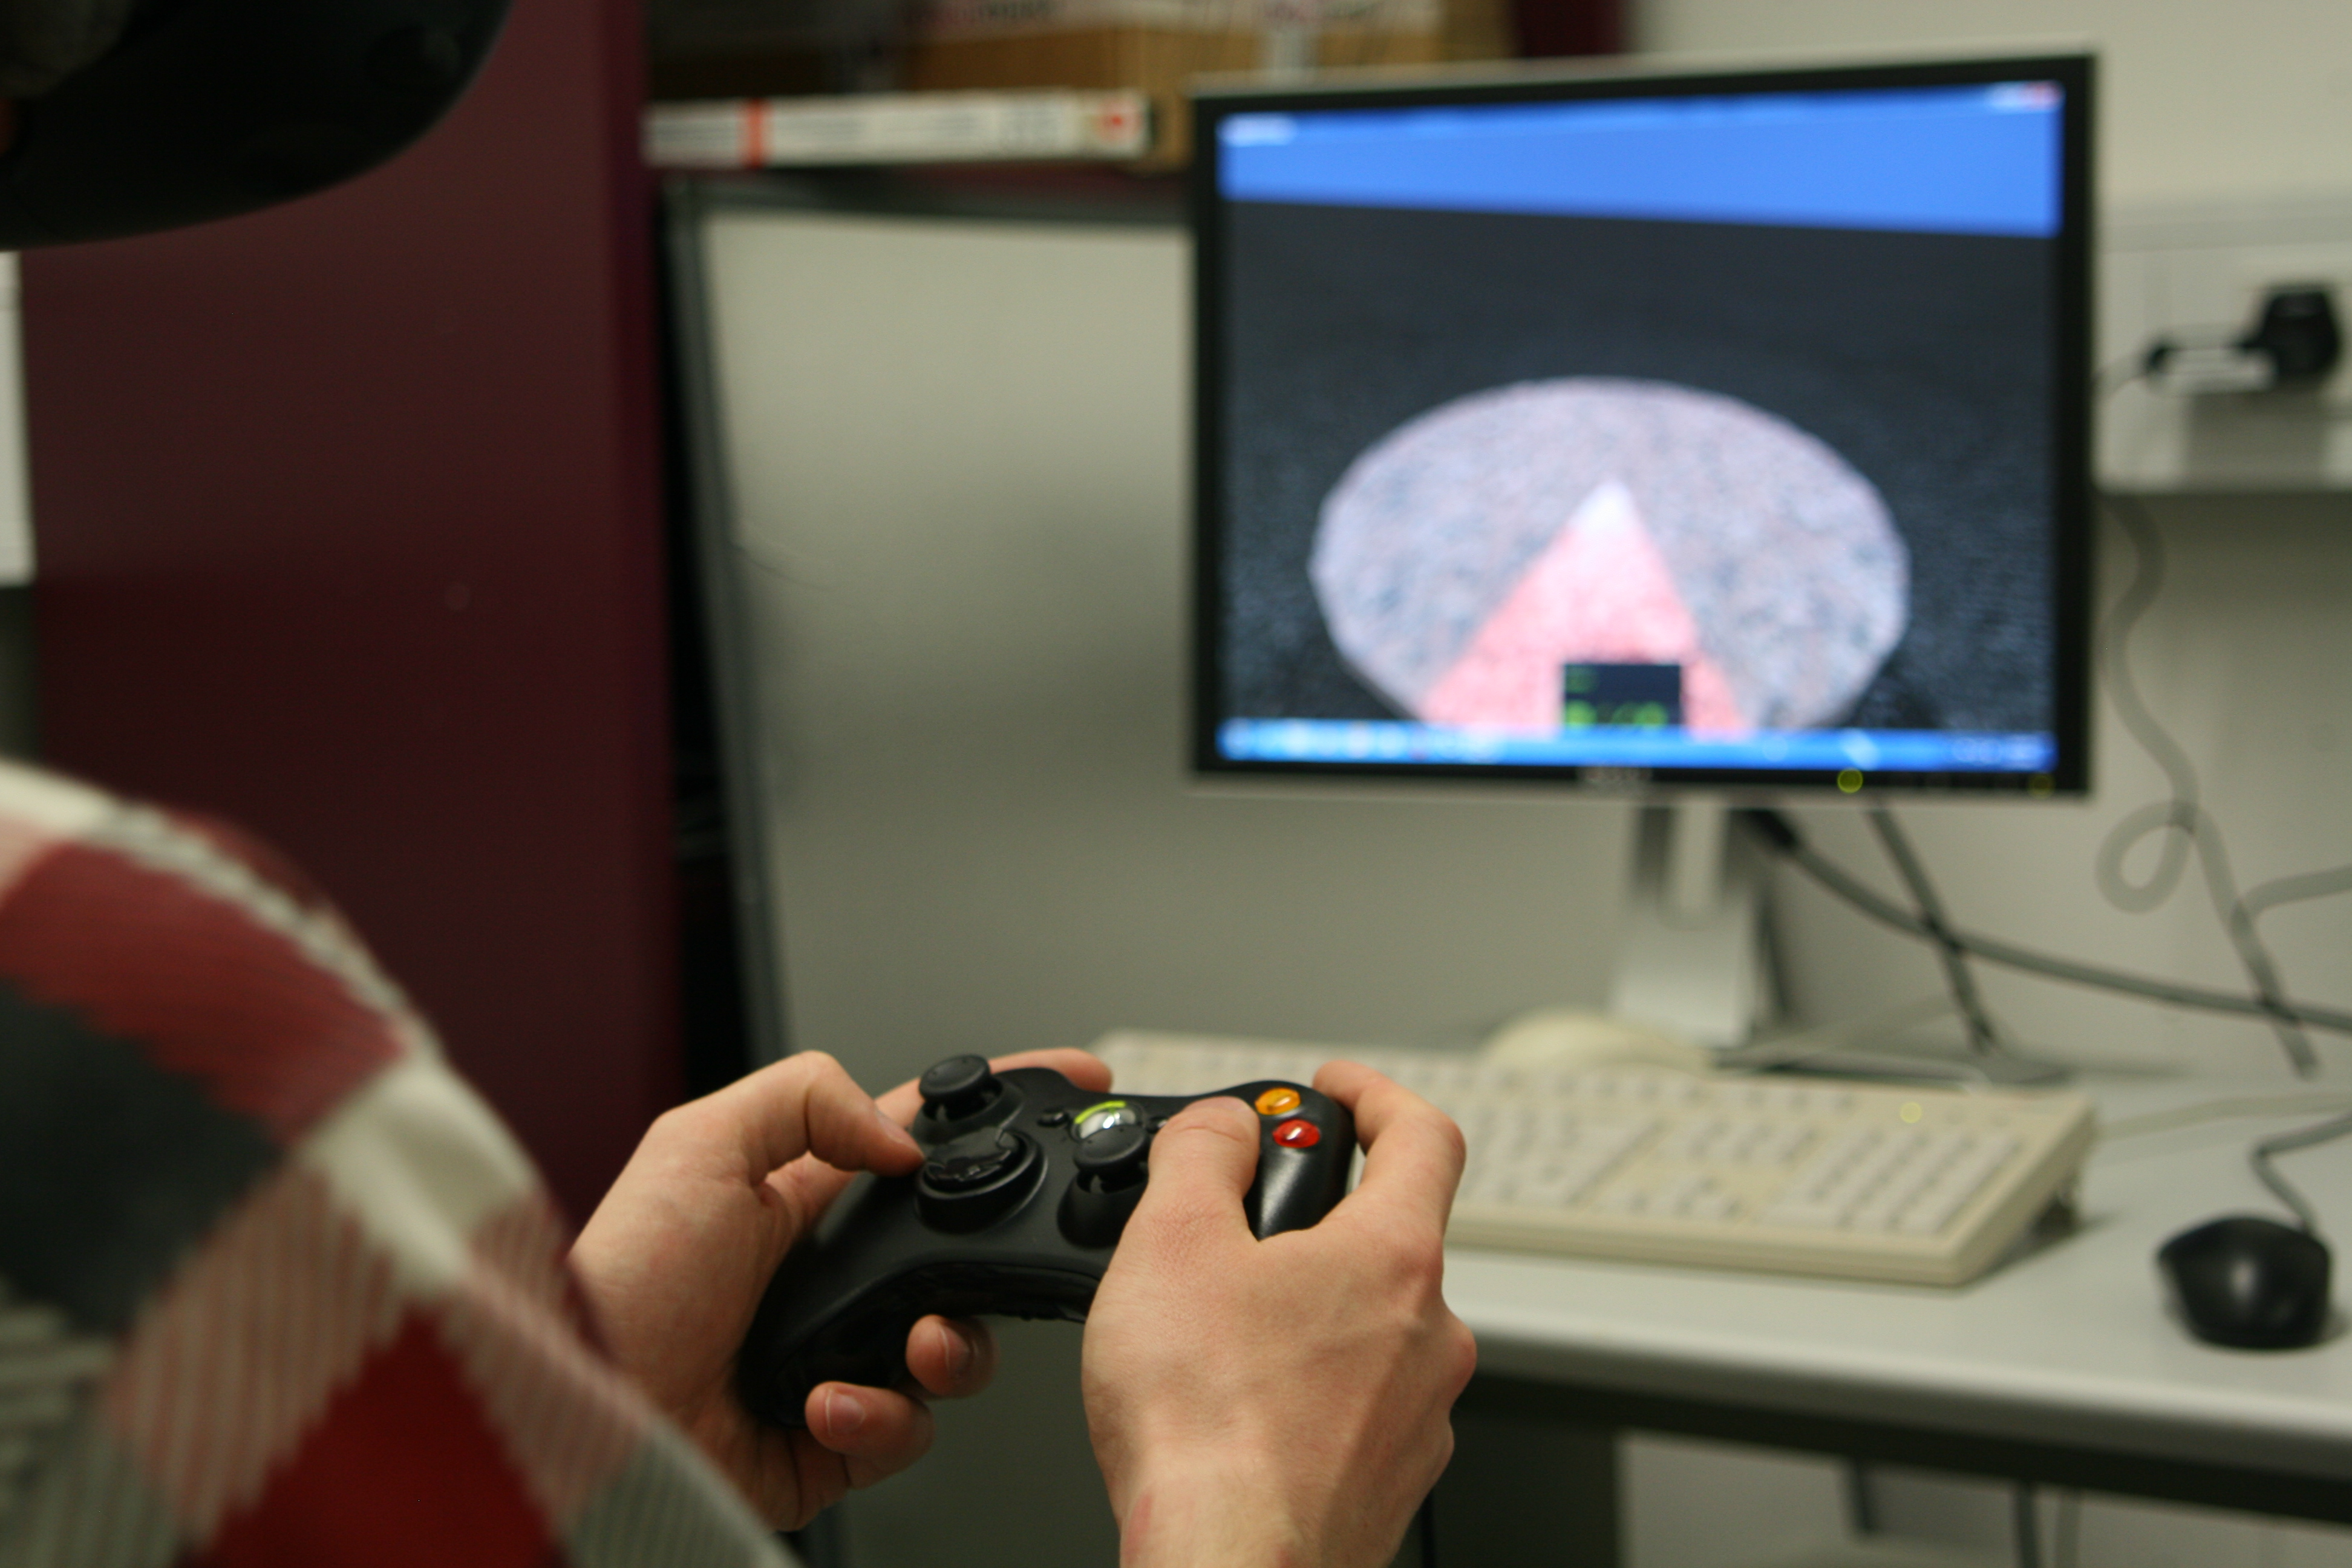
\includegraphics[width=0.5\textwidth]{xbox}
  \caption{XBox controller used to make decisions in the trial phase.} 
  \label{fig:xbox}
\end{figure}

In one part of the experiment (trial phase) the virtual environment consists of a round table and an empty chair which is located at the table and a small blue ball is located on top of the table. In the other part of the experiment (adaptation phase) the virtual environment consists of a square table an there a three different blue objects (a ball, a square and a capsule) located on top of the table. \ref{fig:trial_table}

\begin{figure}
\centering
  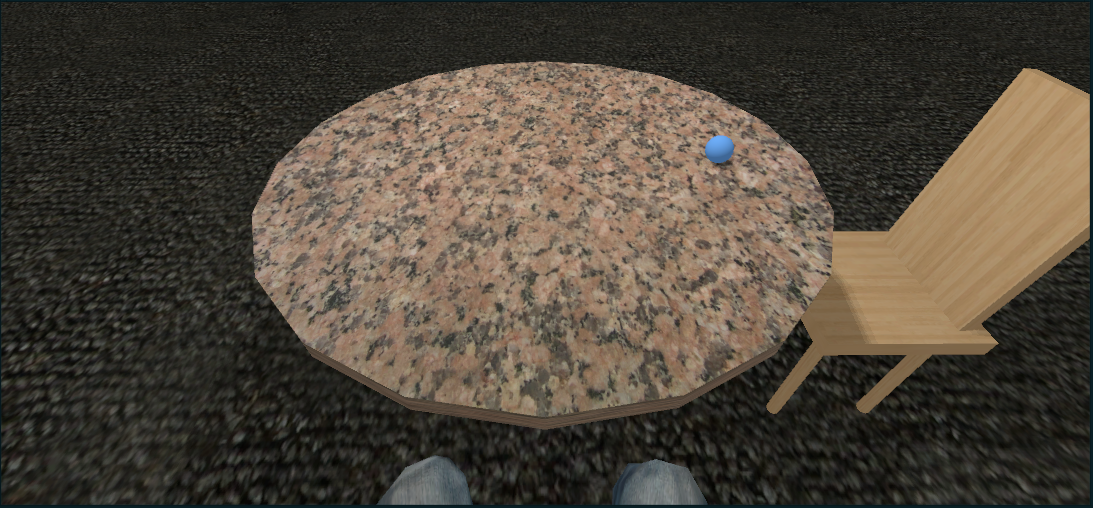
\includegraphics[width=0.5\textwidth]{trial_table}
  \caption{Virtual environment: table with ball and empty chair.} 
  \label{fig:trial_table}
\end{figure}


In the trial phase participants make a decision if they can reach the blue ball by pressing the shoulder buttons of the XBox Controller. The left shoulder button is used to decide that they can not reach the ball and the right shoulder button is used to decide they can reach it. Participants can start each trial by pressing the 'A' button of the XBox controller. In the adaptation phase participants only use their own hand movements to control their virtual arm which is tracked by the HTC Vive controller.

\subsection{Procedure}
The experimenter explained the details of the experiment to each participant before the experiment. Participants will perform a virtual reality task and will wear a head mounted display during the entire experiment. They will sit during the entire experiment and see a round virtual table in front of them. The task will be to judge if they can reach an object that appears on different locations on the table. It is important for the participants to imagine that they can not lean forward to reach the object. Furthermore it is important to make the decision imagining to sit on a chair that appears on different locations around the table for each trial. And sometimes that chair will have their actual location. The usage of the XBox controller was explained like in the section Apparatus. Finally participants were informed that later during the experiment HTC Vive controllers will be used to track their hand movements.

The whole experiment consists of two trial phases and one adaptation phase between the trial phases.

Each trial phase consists of 336 Trials. One trial is to judge if the participant would be able to reach the ball on the table and consists of two steps. First, a red light on the table indicates where an empty chair will appear. The participant confirms the light indicator using the XBox controller. Second, the empty chair appears and the participant decides also via XBox controller if he or she would be able to reach the ball.

In the adaptation phase participants can interact with objects on a square table in a virtual environment similar to the one in the trial phase. In preparation of the adaptation phase the distance between the participants wrists sitting in a T-position is measured. \ref{fig:controller_calibration} The measurement is used as an input variable for the virtual environment to visualize the participant's arm length. There are two conditions (between-subject design,). One group o participants will see a representation of their arm that is only 80\% of their actual arm length and the other group of participants will see a representation of their arm that is 120\% of their actual arm length. In order to control their virtual arm a controller will be attached to the writs of the dominant arm of the participant. \ref{fig:controller_attach} Therefore the virtual arm can mirror the actual movements of the participant. The task in the adaptaion phase is to reach out to 3 objects on the table. The objects disappear if the participant is able to reach them and they remain on the table if the participant is not able to reach them. Participant's are not allowed forward to reach the objects. There 20 repetitions with 3 objects each. \ref{fig:controller_use}.
After the experiment the actual distance of how far participants can reach at table was measured as a reference for further analysis.

\begin{figure}[h]
\centering
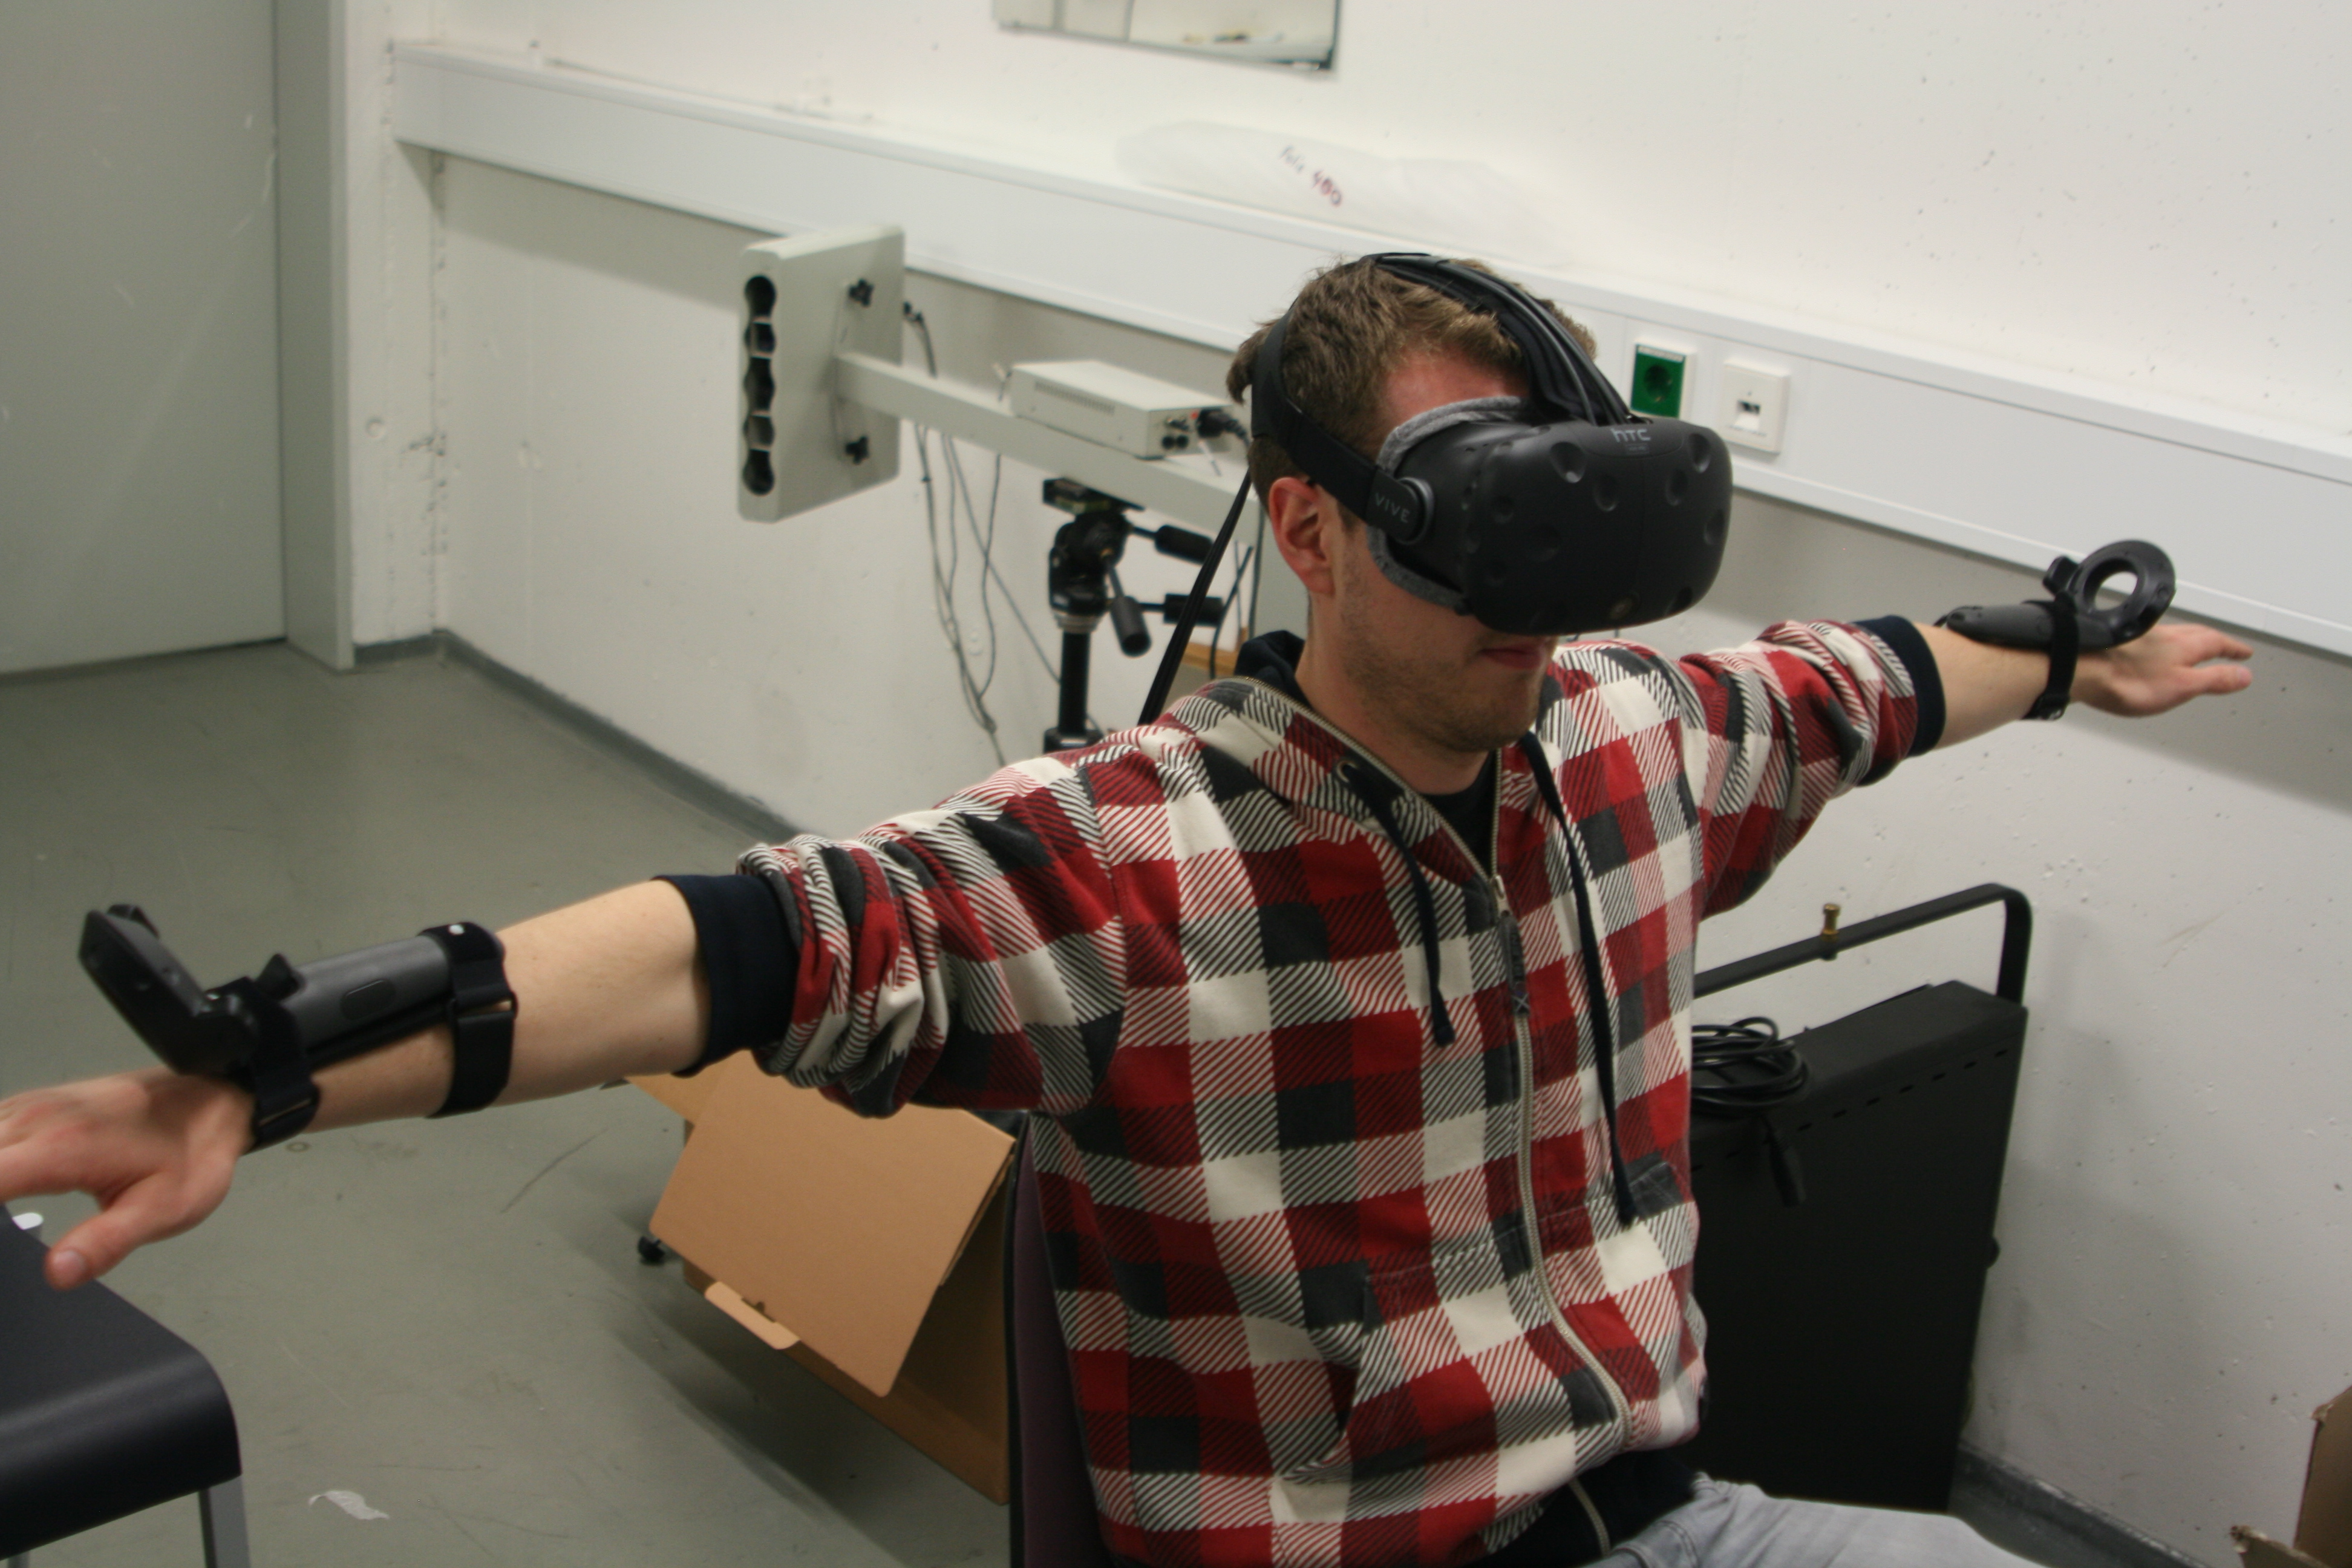
\includegraphics[width=0.5\textwidth]{controller_calibration}
\caption{Two HTC Vive controller attached to the participant's arms to measure and calibrate the virtual arm.}
\label{fig:controller_use}
\end{figure}

\begin{figure}[h]
\centering
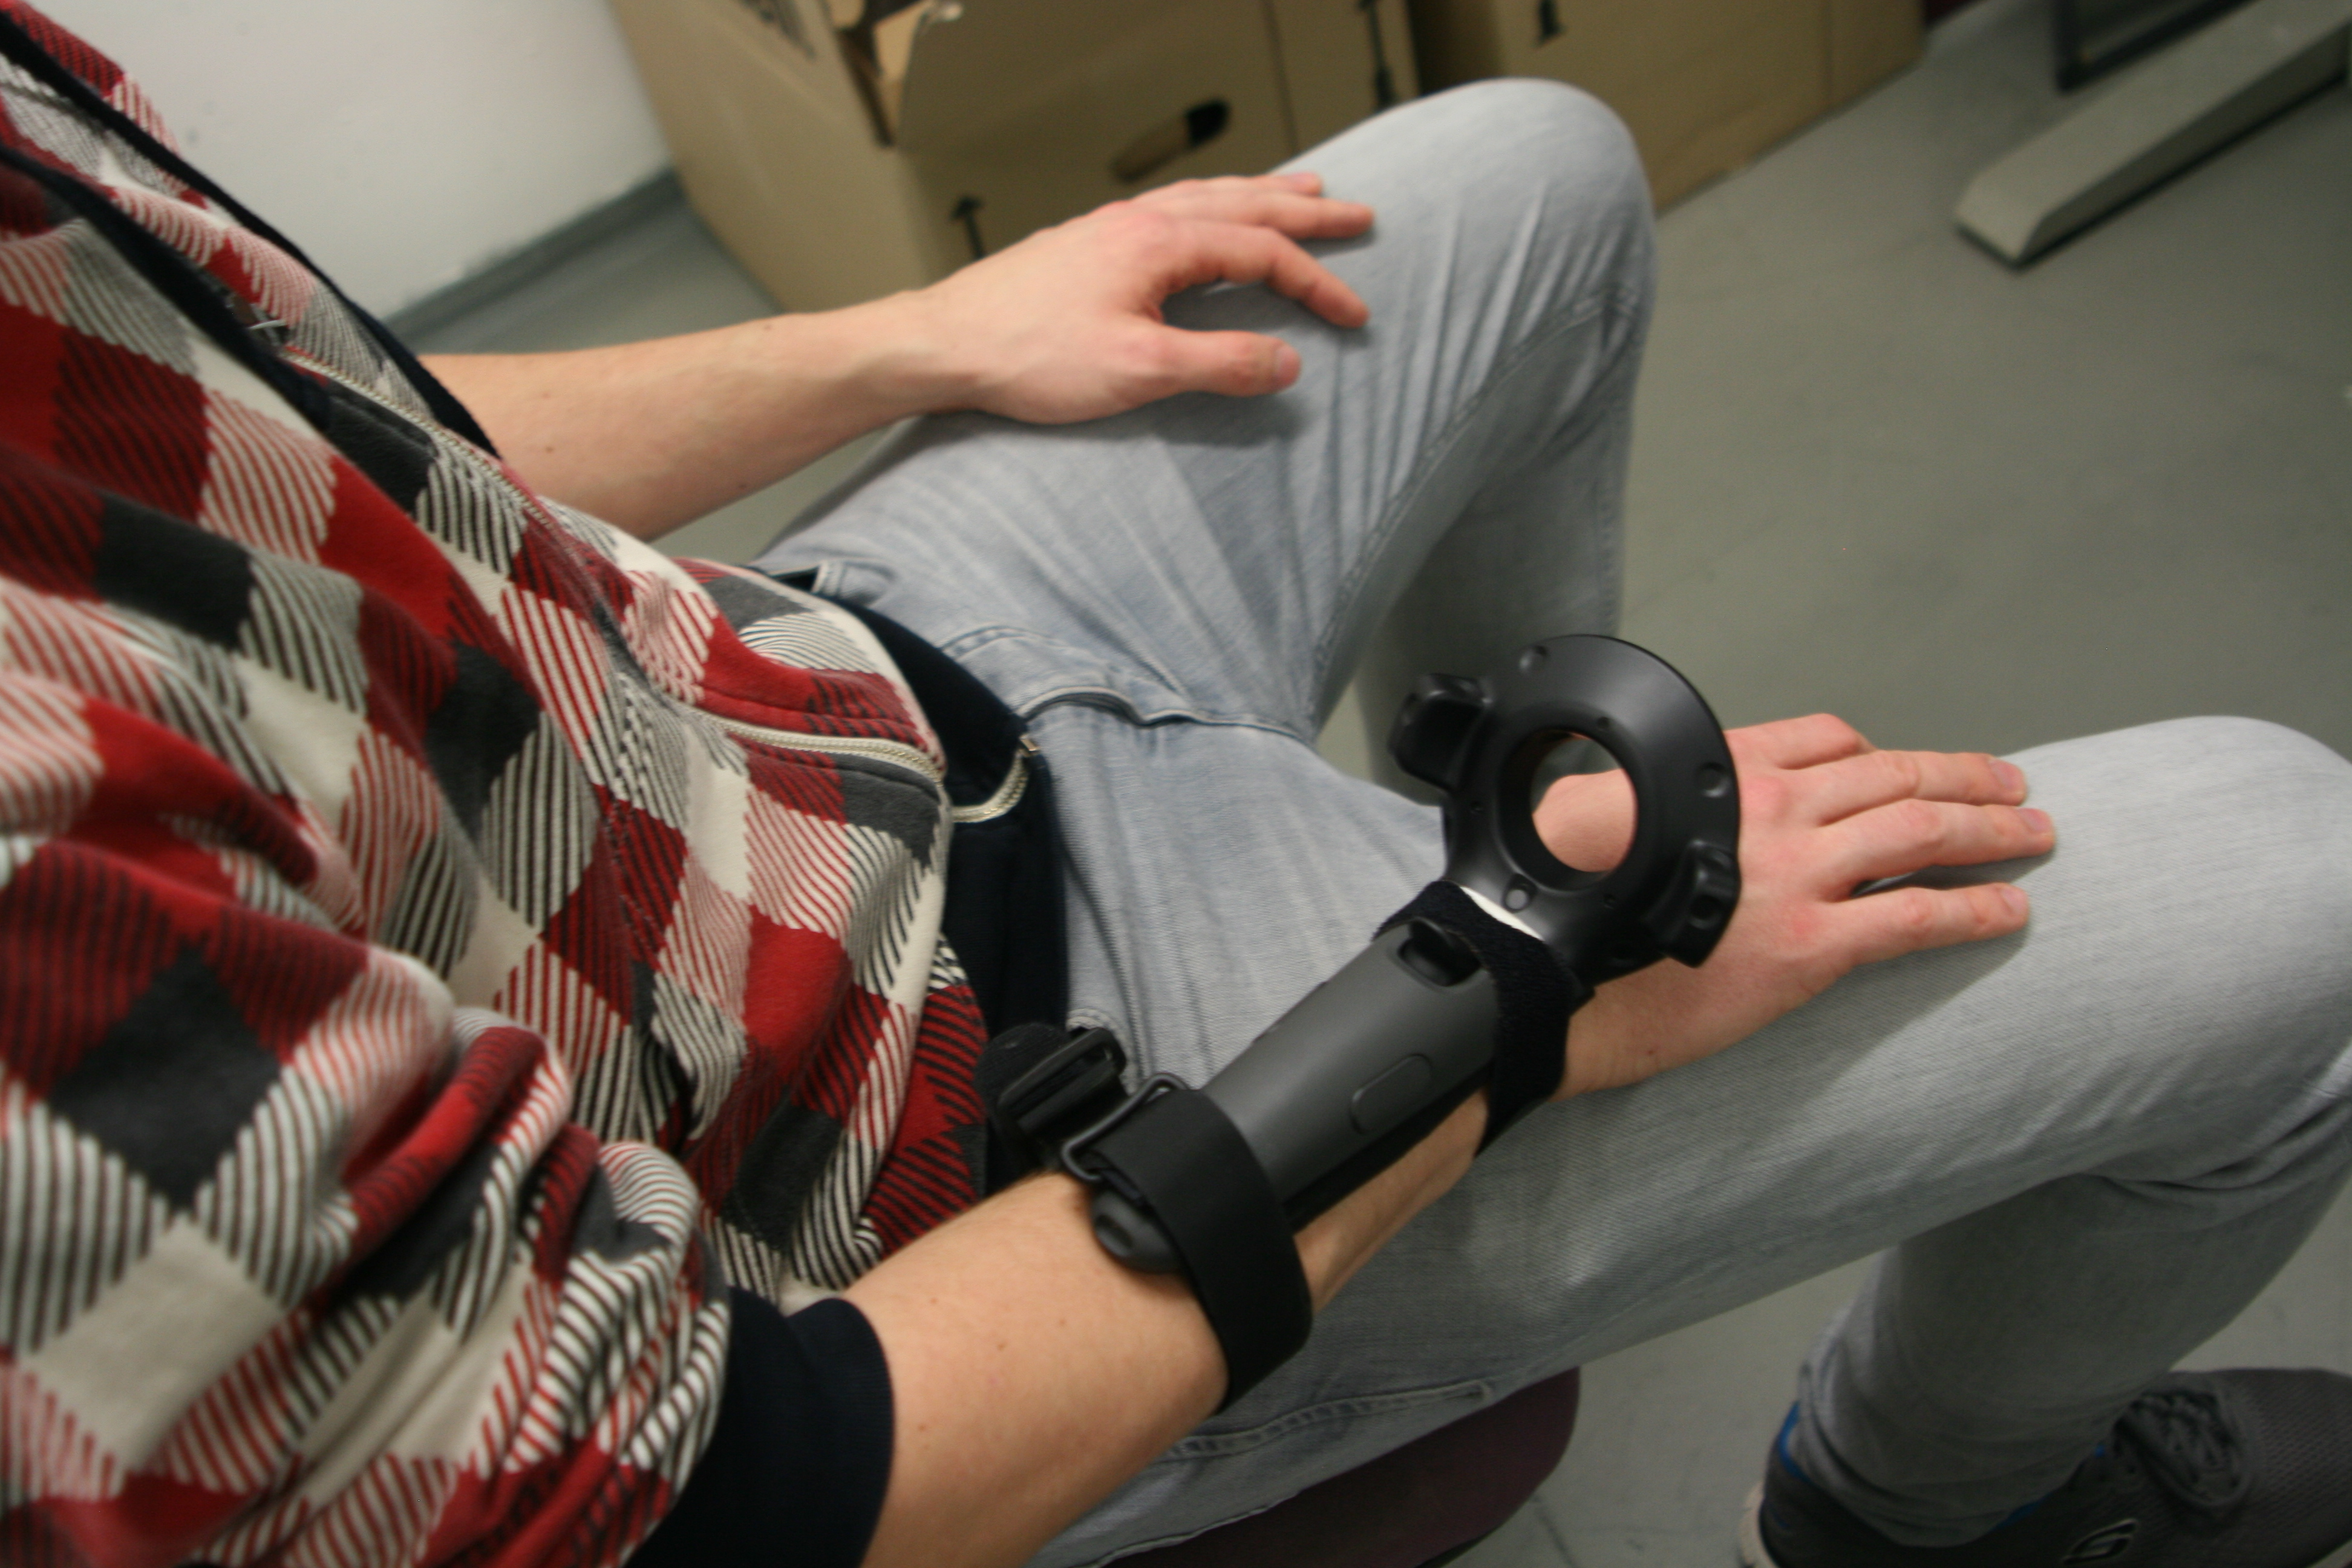
\includegraphics[width=0.5\textwidth]{controller_attach}
\caption{HTC Vive controller attached to the participant's arm to track hand and arm movements.}
\label{fig:controller_calibration}
\end{figure}

\begin{figure}
\centering
  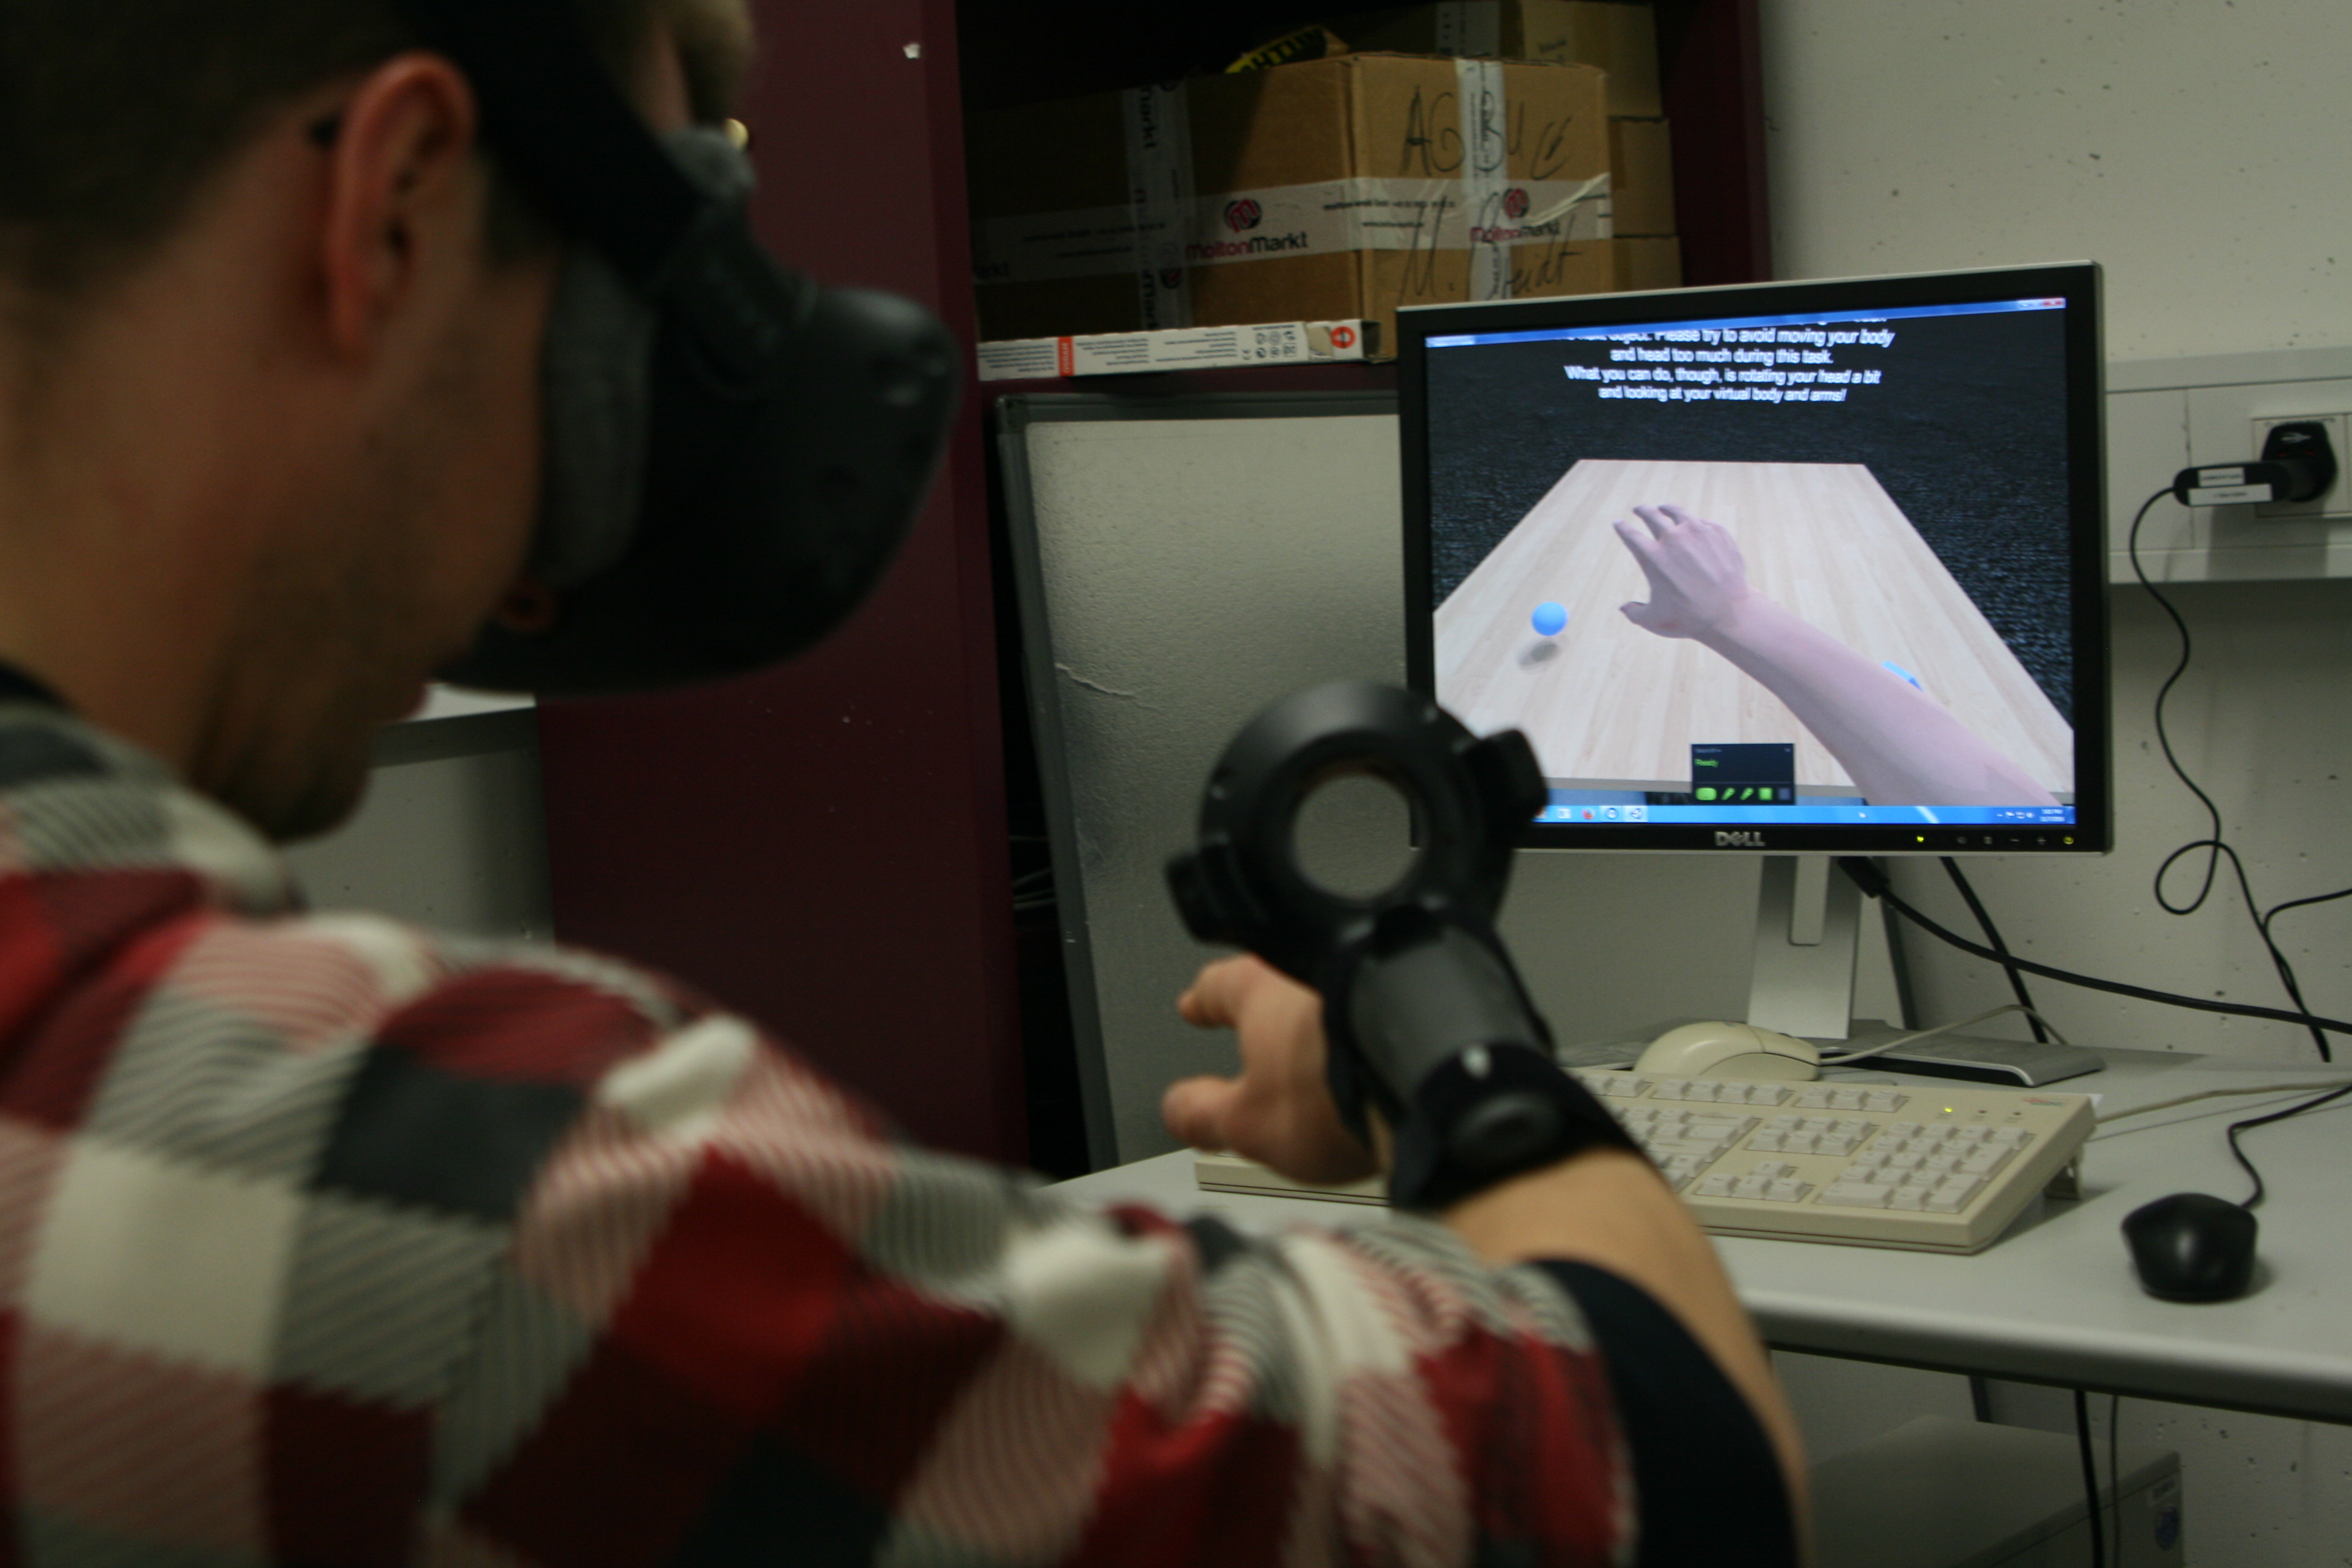
\includegraphics[width=0.5\textwidth]{controller_use}
  \caption{HTC Vive controller attached to the participant's arm to track hand and arm movements.}
  \label{fig:controller_attach}
\end{figure}



%what needs to go in here is:

%instructions that were given to the participants
%training phase (how many trials...)
%counterbalance single / multi (counterbalanced - 10 each side)
